% !TeX TXS-program:bibliography = txs:///biber
\documentclass[14pt, russian]{scrartcl}
\let\counterwithout\relax
\let\counterwithin\relax
%\usepackage{lmodern}
\usepackage{float}
\usepackage{xcolor}
\usepackage{extsizes}
\usepackage{subfig}
\usepackage[export]{adjustbox}
\usepackage{tocvsec2} % возможность менять учитываемую глубину разделов в оглавлении
\usepackage[subfigure]{tocloft}
\usepackage[newfloat]{minted}
\captionsetup[listing]{position=top}

\AtBeginEnvironment{figure}{\vspace{0.5cm}}
\AtBeginEnvironment{table}{\vspace{0.5cm}}
\AtBeginEnvironment{listing}{\vspace{0.5cm}}
\AtBeginEnvironment{algorithm}{\vspace{0.5cm}}
\AtBeginEnvironment{minted}{\vspace{-0.5cm}}

\usepackage{fancyvrb}
\usepackage{ulem,bm,mathrsfs,ifsym} %зачеркивания, особо жирный стиль и RSFS начертание
\usepackage{sectsty} % переопределение стилей подразделов
%%%%%%%%%%%%%%%%%%%%%%%

%%% Поля и разметка страницы %%%
\usepackage{pdflscape}                              % Для включения альбомных страниц
\usepackage{geometry}                               % Для последующего задания полей
\geometry{a4paper,tmargin=2cm,bmargin=2cm,lmargin=3cm,rmargin=1cm} % тоже самое, но лучше

%%% Математические пакеты %%%
\usepackage{amsthm,amsfonts,amsmath,amssymb,amscd}  % Математические дополнения от AMS
\usepackage{mathtools}                              % Добавляет окружение multlined
\usepackage[perpage]{footmisc}
%\usepackage{times}

%%%% Установки для размера шрифта 14 pt %%%%
%% Формирование переменных и констант для сравнения (один раз для всех подключаемых файлов)%%
%% должно располагаться до вызова пакета fontspec или polyglossia, потому что они сбивают его работу
%\newlength{\curtextsize}
%\newlength{\bigtextsize}
%\setlength{\bigtextsize}{13pt}
\KOMAoptions{fontsize=14pt}

\makeatletter
\def\showfontsize{\f@size{} point}
\makeatother

%\makeatletter
%\show\f@size                                       % неплохо для отслеживания, но вызывает стопорение процесса, если документ компилируется без команды  -interaction=nonstopmode 
%\setlength{\curtextsize}{\f@size pt}
%\makeatother

%шрифт times
\usepackage{tempora}
%\usepackage{pscyr}
%\setmainfont[Ligatures={TeX,Historic}]{Times New Roman}

   %%% Решение проблемы копирования текста в буфер кракозябрами
%    \input glyphtounicode.tex
%    \input glyphtounicode-cmr.tex %from pdfx package
%    \pdfgentounicode=1
    \usepackage{cmap}                               % Улучшенный поиск русских слов в полученном pdf-файле
    \usepackage[T1]{fontenc}                       % Поддержка русских букв
    \usepackage[utf8]{inputenc}                     % Кодировка utf8
    \usepackage[english, main=russian]{babel}            % Языки: русский, английский
%   \IfFileExists{pscyr.sty}{\usepackage{pscyr}}{}  % Красивые русские шрифты
%\renewcommand{\rmdefault}{ftm}
%%% Оформление абзацев %%%
\usepackage{indentfirst}                            % Красная строка
%\usepackage{eskdpz}

%%% Таблицы %%%
\usepackage{longtable}                              % Длинные таблицы
\usepackage{multirow,makecell,array}                % Улучшенное форматирование таблиц
\usepackage{booktabs}                               % Возможность оформления таблиц в классическом книжном стиле (при правильном использовании не противоречит ГОСТ)

%%% Общее форматирование
\usepackage{soulutf8}                               % Поддержка переносоустойчивых подчёркиваний и зачёркиваний
\usepackage{icomma}                                 % Запятая в десятичных дробях



%%% Изображения %%%
\usepackage{graphicx}                               % Подключаем пакет работы с графикой
\usepackage{wrapfig}

%%% Списки %%%
\usepackage{enumitem}

%%% Подписи %%%
\usepackage{caption}                                % Для управления подписями (рисунков и таблиц) % Может управлять номерами рисунков и таблиц с caption %Иногда может управлять заголовками в списках рисунков и таблиц
%% Использование:
%\begin{table}[h!]\ContinuedFloat - чтобы не переключать счетчик
%\captionsetup{labelformat=continued}% должен стоять до самого caption
%\caption{}
% либо ручками \caption*{Продолжение таблицы~\ref{...}.} :)

%%% Интервалы %%%
\addto\captionsrussian{%
  \renewcommand{\listingname}{Листинг}%
}
%%% Счётчики %%%
\usepackage[figure,table,section]{totalcount}               % Счётчик рисунков и таблиц
\DeclareTotalCounter{lstlisting}
\usepackage{totcount}                               % Пакет создания счётчиков на основе последнего номера подсчитываемого элемента (может требовать дважды компилировать документ)
\usepackage{totpages}                               % Счётчик страниц, совместимый с hyperref (ссылается на номер последней страницы). Желательно ставить последним пакетом в преамбуле

%%% Продвинутое управление групповыми ссылками (пока только формулами) %%%
%% Кодировки и шрифты %%%

%   \newfontfamily{\cyrillicfont}{Times New Roman}
%   \newfontfamily{\cyrillicfonttt}{CMU Typewriter Text}
	%\setmainfont{Times New Roman}
	%\newfontfamily\cyrillicfont{Times New Roman}
	%\setsansfont{Times New Roman}                    %% задаёт шрифт без засечек
%	\setmonofont{Liberation Mono}               %% задаёт моноширинный шрифт
%    \IfFileExists{pscyr.sty}{\renewcommand{\rmdefault}{ftm}}{}
%%% Интервалы %%%
%linespread-реализация ближе к реализации полуторного интервала в ворде.
%setspace реализация заточена под шрифты 10, 11, 12pt, под остальные кегли хуже, но всё же ближе к типографской классике. 
\linespread{1.3}                    % Полуторный интервал (ГОСТ Р 7.0.11-2011, 5.3.6)
%\renewcommand{\@biblabel}[1]{#1}

%%% Гиперссылки %%%
\usepackage{hyperref}

%%% Выравнивание и переносы %%%
\sloppy                             % Избавляемся от переполнений
\clubpenalty=10000                  % Запрещаем разрыв страницы после первой строки абзаца
\widowpenalty=10000                 % Запрещаем разрыв страницы после последней строки абзаца

\makeatletter % малые заглавные, small caps shape
\let\@@scshape=\scshape
\renewcommand{\scshape}{%
  \ifnum\strcmp{\f@series}{bx}=\z@
    \usefont{T1}{cmr}{bx}{sc}%
  \else
    \ifnum\strcmp{\f@shape}{it}=\z@
      \fontshape{scsl}\selectfont
    \else
      \@@scshape
    \fi
  \fi}
\makeatother

%%% Подписи %%%
%\captionsetup{%
%singlelinecheck=off,                % Многострочные подписи, например у таблиц
%skip=2pt,                           % Вертикальная отбивка между подписью и содержимым рисунка или таблицы определяется ключом
%justification=centering,            % Центрирование подписей, заданных командой \caption
%}
%%%        Подключение пакетов                 %%%
\usepackage{ifthen}                 % добавляет ifthenelse
%%% Инициализирование переменных, не трогать!  %%%
\newcounter{intvl}
\newcounter{otstup}
\newcounter{contnumeq}
\newcounter{contnumfig}
\newcounter{contnumtab}
\newcounter{pgnum}
\newcounter{bibliosel}
\newcounter{chapstyle}
\newcounter{headingdelim}
\newcounter{headingalign}
\newcounter{headingsize}
\newcounter{tabcap}
\newcounter{tablaba}
\newcounter{tabtita}
%%%%%%%%%%%%%%%%%%%%%%%%%%%%%%%%%%%%%%%%%%%%%%%%%%

%%% Область упрощённого управления оформлением %%%

%% Интервал между заголовками и между заголовком и текстом
% Заголовки отделяют от текста сверху и снизу тремя интервалами (ГОСТ Р 7.0.11-2011, 5.3.5)
\setcounter{intvl}{3}               % Коэффициент кратности к размеру шрифта

%% Отступы у заголовков в тексте
\setcounter{otstup}{0}              % 0 --- без отступа; 1 --- абзацный отступ

%% Нумерация формул, таблиц и рисунков
\setcounter{contnumeq}{1}           % Нумерация формул: 0 --- пораздельно (во введении подряд, без номера раздела); 1 --- сквозная нумерация по всей диссертации
\setcounter{contnumfig}{1}          % Нумерация рисунков: 0 --- пораздельно (во введении подряд, без номера раздела); 1 --- сквозная нумерация по всей диссертации
\setcounter{contnumtab}{1}          % Нумерация таблиц: 0 --- пораздельно (во введении подряд, без номера раздела); 1 --- сквозная нумерация по всей диссертации

%% Оглавление
\setcounter{pgnum}{0}               % 0 --- номера страниц никак не обозначены; 1 --- Стр. над номерами страниц (дважды компилировать после изменения)

%% Библиография
\setcounter{bibliosel}{1}           % 0 --- встроенная реализация с загрузкой файла через движок bibtex8; 1 --- реализация пакетом biblatex через движок biber

%% Текст и форматирование заголовков
\setcounter{chapstyle}{1}           % 0 --- разделы только под номером; 1 --- разделы с названием "Глава" перед номером
\setcounter{headingdelim}{1}        % 0 --- номер отделен пропуском в 1em или \quad; 1 --- номера разделов и приложений отделены точкой с пробелом, подразделы пропуском без точки; 2 --- номера разделов, подразделов и приложений отделены точкой с пробелом.

%% Выравнивание заголовков в тексте
\setcounter{headingalign}{0}        % 0 --- по центру; 1 --- по левому краю

%% Размеры заголовков в тексте
\setcounter{headingsize}{0}         % 0 --- по ГОСТ, все всегда 14 пт; 1 --- пропорционально изменяющийся размер в зависимости от базового шрифта

%% Подпись таблиц
\setcounter{tabcap}{0}              % 0 --- по ГОСТ, номер таблицы и название разделены тире, выровнены по левому краю, при необходимости на нескольких строках; 1 --- подпись таблицы не по ГОСТ, на двух и более строках, дальнейшие настройки: 
%Выравнивание первой строки, с подписью и номером
\setcounter{tablaba}{2}             % 0 --- по левому краю; 1 --- по центру; 2 --- по правому краю
%Выравнивание строк с самим названием таблицы
\setcounter{tabtita}{1}             % 0 --- по левому краю; 1 --- по центру; 2 --- по правому краю

%%% Рисунки %%%
\DeclareCaptionLabelSeparator*{emdash}{~--- }             % (ГОСТ 2.105, 4.3.1)
\captionsetup[figure]{labelsep=emdash,font=onehalfspacing,position=bottom}

%%% Таблицы %%%
\ifthenelse{\equal{\thetabcap}{0}}{%
    \newcommand{\tabcapalign}{\raggedright}  % по левому краю страницы или аналога parbox
}

\ifthenelse{\equal{\thetablaba}{0} \AND \equal{\thetabcap}{1}}{%
    \newcommand{\tabcapalign}{\raggedright}  % по левому краю страницы или аналога parbox
}

\ifthenelse{\equal{\thetablaba}{1} \AND \equal{\thetabcap}{1}}{%
    \newcommand{\tabcapalign}{\centering}    % по центру страницы или аналога parbox
}

\ifthenelse{\equal{\thetablaba}{2} \AND \equal{\thetabcap}{1}}{%
    \newcommand{\tabcapalign}{\raggedleft}   % по правому краю страницы или аналога parbox
}

\ifthenelse{\equal{\thetabtita}{0} \AND \equal{\thetabcap}{1}}{%
    \newcommand{\tabtitalign}{\raggedright}  % по левому краю страницы или аналога parbox
}

\ifthenelse{\equal{\thetabtita}{1} \AND \equal{\thetabcap}{1}}{%
    \newcommand{\tabtitalign}{\centering}    % по центру страницы или аналога parbox
}

\ifthenelse{\equal{\thetabtita}{2} \AND \equal{\thetabcap}{1}}{%
    \newcommand{\tabtitalign}{\raggedleft}   % по правому краю страницы или аналога parbox
}

\DeclareCaptionFormat{tablenocaption}{\tabcapalign #1\strut}        % Наименование таблицы отсутствует
\ifthenelse{\equal{\thetabcap}{0}}{%
    \DeclareCaptionFormat{tablecaption}{\tabcapalign #1#2#3}
    \captionsetup[table]{labelsep=emdash}                       % тире как разделитель идентификатора с номером от наименования
}{%
    \DeclareCaptionFormat{tablecaption}{\tabcapalign #1#2\par%  % Идентификатор таблицы на отдельной строке
        \tabtitalign{#3}}                                       % Наименование таблицы строкой ниже
    \captionsetup[table]{labelsep=space}                        % пробельный разделитель идентификатора с номером от наименования
}
\captionsetup[table]{format=tablecaption,singlelinecheck=off,font=onehalfspacing,position=top,skip=-5pt}  % многострочные наименования и прочее
\DeclareCaptionLabelFormat{continued}{Продолжение таблицы~#2}
\setlength{\belowcaptionskip}{.2cm}
\setlength{\intextsep}{0ex}

%%% Подписи подрисунков %%%
\renewcommand{\thesubfigure}{\asbuk{subfigure}}           % Буквенные номера подрисунков
\captionsetup[subfigure]{font={normalsize},               % Шрифт подписи названий подрисунков (не отличается от основного)
    labelformat=brace,                                    % Формат обозначения подрисунка
    justification=centering,                              % Выключка подписей (форматирование), один из вариантов            
}
%\DeclareCaptionFont{font12pt}{\fontsize{12pt}{13pt}\selectfont} % объявляем шрифт 12pt для использования в подписях, тут же надо интерлиньяж объявлять, если не наследуется
%\captionsetup[subfigure]{font={font12pt}}                 % Шрифт подписи названий подрисунков (всегда 12pt)

%%% Настройки гиперссылок %%%

\definecolor{linkcolor}{rgb}{0.0,0,0}
\definecolor{citecolor}{rgb}{0,0.0,0}
\definecolor{urlcolor}{rgb}{0,0,0}

\hypersetup{
    linktocpage=true,           % ссылки с номера страницы в оглавлении, списке таблиц и списке рисунков
%    linktoc=all,                % both the section and page part are links
%    pdfpagelabels=false,        % set PDF page labels (true|false)
    plainpages=true,           % Forces page anchors to be named by the Arabic form  of the page number, rather than the formatted form
    colorlinks,                 % ссылки отображаются раскрашенным текстом, а не раскрашенным прямоугольником, вокруг текста
    linkcolor={linkcolor},      % цвет ссылок типа ref, eqref и подобных
    citecolor={citecolor},      % цвет ссылок-цитат
    urlcolor={urlcolor},        % цвет гиперссылок
    pdflang={ru},
}
\urlstyle{same}
%%% Шаблон %%%
%\DeclareRobustCommand{\todo}{\textcolor{red}}       % решаем проблему превращения названия цвета в результате \MakeUppercase, http://tex.stackexchange.com/a/187930/79756 , \DeclareRobustCommand protects \todo from expanding inside \MakeUppercase
\setlength{\parindent}{2.5em}                       % Абзацный отступ. Должен быть одинаковым по всему тексту и равен пяти знакам (ГОСТ Р 7.0.11-2011, 5.3.7).

%%% Списки %%%
% Используем дефис для ненумерованных списков (ГОСТ 2.105-95, 4.1.7)
%\renewcommand{\labelitemi}{\normalfont\bfseries~{---}} 
\renewcommand{\labelitemi}{\bfseries~{---}} 
\setlist{nosep,%                                    % Единый стиль для всех списков (пакет enumitem), без дополнительных интервалов.
    labelindent=\parindent,leftmargin=*%            % Каждый пункт, подпункт и перечисление записывают с абзацного отступа (ГОСТ 2.105-95, 4.1.8)
}
%%%%%%%%%%%%%%%%%%%%%%
%\usepackage{xltxtra} % load xunicode

\usepackage{ragged2e}
\usepackage[explicit]{titlesec}
\usepackage{placeins}
\usepackage{xparse}
\usepackage{csquotes}

\usepackage{listingsutf8}
\usepackage{url} %пакеты расширений
\usepackage{algorithm, algorithmicx}
\usepackage[noend]{algpseudocode}
\usepackage{blkarray}
\usepackage{chngcntr}
\usepackage{tabularx}
\usepackage[backend=biber, 
    bibstyle=gost-numeric,
    citestyle=nature]{biblatex}
\newcommand*\template[1]{\text{<}#1\text{>}}
\addbibresource{biblio.bib}
  
\titleformat{name=\section,numberless}[block]{\normalfont\Large\centering}{}{0em}{#1}
\titleformat{\section}[block]{\normalfont\Large\bfseries\raggedright}{}{0em}{\thesection\hspace{0.25em}#1}
\titleformat{\subsection}[block]{\normalfont\Large\bfseries\raggedright}{}{0em}{\thesubsection\hspace{0.25em}#1}
\titleformat{\subsubsection}[block]{\normalfont\large\bfseries\raggedright}{}{0em}{\thesubsubsection\hspace{0.25em}#1}

\let\Algorithm\algorithm
\renewcommand\algorithm[1][]{\Algorithm[#1]\setstretch{1.5}}
%\renewcommand{\listingscaption}{Листинг}

\usepackage{pifont}
\usepackage{calc}
\usepackage{suffix}
\usepackage{csquotes}
\DeclareQuoteStyle{russian}
    {\guillemotleft}{\guillemotright}[0.025em]
    {\quotedblbase}{\textquotedblleft}
\ExecuteQuoteOptions{style=russian}
\newcommand{\enq}[1]{\enquote{#1}}  
\newcommand{\eng}[1]{\begin{english}#1\end{english}}
% Подчиненные счетчики в окружениях http://old.kpfu.ru/journals/izv_vuz/arch/sample1251.tex
\newcounter{cTheorem} 
\newcounter{cDefinition}
\newcounter{cConsequent}
\newcounter{cExample}
\newcounter{cLemma}
\newcounter{cConjecture}
\newtheorem{Theorem}{Теорема}[cTheorem]
\newtheorem{Definition}{Определение}[cDefinition]
\newtheorem{Consequent}{Следствие}[cConsequent]
\newtheorem{Example}{Пример}[cExample]
\newtheorem{Lemma}{Лемма}[cLemma]
\newtheorem{Conjecture}{Гипотеза}[cConjecture]

\renewcommand{\theTheorem}{\arabic{Theorem}}
\renewcommand{\theDefinition}{\arabic{Definition}}
\renewcommand{\theConsequent}{\arabic{Consequent}}
\renewcommand{\theExample}{\arabic{Example}}
\renewcommand{\theLemma}{\arabic{Lemma}}
\renewcommand{\theConjecture}{\arabic{Conjecture}}
%\makeatletter
\NewDocumentCommand{\Newline}{}{\text{\\}}
\newcommand{\sequence}[2]{\ensuremath \left(#1,\ \dots,\ #2\right)}

\definecolor{mygreen}{rgb}{0,0.6,0}
\definecolor{mygray}{rgb}{0.5,0.5,0.5}
\definecolor{mymauve}{rgb}{0.58,0,0.82}
\renewcommand{\listalgorithmname}{Список алгоритмов}
\floatname{algorithm}{Листинг}
\renewcommand{\lstlistingname}{Листинг}
\renewcommand{\thealgorithm}{\arabic{algorithm}}

\newcommand{\refAlgo}[1]{(листинг \ref{#1})}
\newcommand{\refImage}[1]{(рисунок \ref{#1})}

\renewcommand{\theenumi}{\arabic{enumi}.}% Меняем везде перечисления на цифра.цифра	
\renewcommand{\labelenumi}{\arabic{enumi}.}% Меняем везде перечисления на цифра.цифра
\renewcommand{\theenumii}{\arabic{enumii}}% Меняем везде перечисления на цифра.цифра
\renewcommand{\labelenumii}{(\arabic{enumii})}% Меняем везде перечисления на цифра.цифра
\renewcommand{\theenumiii}{\roman{enumiii}}% Меняем везде перечисления на цифра.цифра
\renewcommand{\labelenumiii}{(\roman{enumiii})}% Меняем везде перечисления на цифра.цифра
%\newfontfamily\AnkaCoder[Path=src/fonts/]{AnkaCoder-r.ttf}
\renewcommand{\labelitemi}{---}
\renewcommand{\labelitemii}{---}

%\usepackage{courier}

\lstdefinelanguage{Refal}{
  alsodigit = {.,<,>},
  morekeywords = [1]{$ENTRY},
  morekeywords = [2]{Go, Put, Get, Open, Close, Arg, Add, Sub, Mul, Div, Symb, Explode, Implode},
  %keyword4
  morekeywords = [3]{<,>},
  %keyword5
  morekeywords = [4]{e.,t.,s.},
  sensitive = true,
  morecomment = [l]{*},
  morecomment = [s]{/*}{*/},
  commentstyle = \color{mygreen},
  morestring = [b]",
  morestring = [b]',
  stringstyle = \color{purple}
}

\makeatletter
\def\p@subsection{}
\def\p@subsubsection{\thesection\,\thesubsection\,}
\makeatother
\newcommand{\prog}[1]{{\ttfamily\small#1}}
\lstset{ %
  backgroundcolor=\color{white},   % choose the background color; you must add \usepackage{color} or \usepackage{xcolor}
  basicstyle=\ttfamily\footnotesize, 
  %basicstyle=\footnotesize\AnkaCoder,        % the size of the fonts that are used for the code
  breakatwhitespace=false,         % sets if automatic breaks shoulbd only happen at whitespace
  breaklines=true,                 % sets automatic line breaking
  captionpos=top,                    % sets the caption-position to bottom
  commentstyle=\color{mygreen},    % comment style
  deletekeywords={...},            % if you want to delete keywords from the given language
  escapeinside={\%*}{*)},          % if you want to add LaTeX within your code
  extendedchars=true,              % lets you use non-ASCII characters; for 8-bits encodings only, does not work with UTF-8
  inputencoding=utf8,
  frame=single,                    % adds a frame around the code
  keepspaces=true,                 % keeps spaces in text, useful for keeping indentation of code (possibly needs columns=flexible)
  keywordstyle=\bf,       % keyword style
  language=Refal,                    % the language of the code
  morekeywords={<,>,$ENTRY,Go,Arg, Open, Close, e., s., t., Get, Put}, 
  							       % if you want to add more keywords to the set
  numbers=left,                    % where to put the line-numbers; possible values are (none, left, right)
  numbersep=5pt,                   % how far the line-numbers are from the code
  xleftmargin=25pt,
  xrightmargin=25pt,
  numberstyle=\small\color{black}, % the style that is used for the line-numbers
  rulecolor=\color{black},         % if not set, the frame-color may be changed on line-breaks within not-black text (e.g. comments (green here))
  showspaces=false,                % show spaces everywhere adding particular underscores; it overrides 'showstringspaces'
  showstringspaces=false,          % underline spaces within strings only
  showtabs=false,                  % show tabs within strings adding particular underscores
  stepnumber=1,                    % the step between two line-numbers. If it's 1, each line will be numbered
  stringstyle=\color{mymauve},     % string literal style
  tabsize=8,                       % sets default tabsize to 8 spaces
  title=\lstname                   % show the filename of files included with \lstinputlisting; also try caption instead of title
}
\newcommand{\anonsection}[1]{\cleardoublepage
\phantomsection
\addcontentsline{toc}{section}{\protect\numberline{}#1}
\section*{#1}\vspace*{2.5ex} % По госту положены 3 пустые строки после заголовка ненумеруемого раздела
}
\newcommand{\sectionbreak}{\clearpage}
\renewcommand{\sectionfont}{\normalsize} % Сбиваем стиль оглавления в стандартный
\renewcommand{\cftsecleader}{\cftdotfill{\cftdotsep}} % Точки в оглавлении напротив разделов

\renewcommand{\cftsecfont}{\normalfont\large} % Переключение на times в содержании
\renewcommand{\cftsubsecfont}{\normalfont\large} % Переключение на times в содержании

\usepackage{caption} 
%\captionsetup[table]{justification=raggedleft} 
%\captionsetup[figure]{justification=centering,labelsep=endash}
\usepackage{amsmath}    % \bar    (матрицы и проч. ...)
\usepackage{amsfonts}   % \mathbb (символ для множества действительных чисел и проч. ...)
\usepackage{mathtools}  % \abs, \norm
    \DeclarePairedDelimiter\abs{\lvert}{\rvert} % операция модуля
    \DeclarePairedDelimiter\norm{\lVert}{\rVert} % операция нормы
\DeclareTextCommandDefault{\textvisiblespace}{%
  \mbox{\kern.06em\vrule \@height.3ex}%
  \vbox{\hrule \@width.3em}%
  \hbox{\vrule \@height.3ex}}    
\newsavebox{\spacebox}
\begin{lrbox}{\spacebox}
\verb*! !
\end{lrbox}
\newcommand{\aspace}{\usebox{\spacebox}}
\DeclareTotalCounter{listing}

\makeatletter
\renewcommand*{\p@subsubsection}{}
\makeatother
    
\begin{document}
\sloppy

\def\figurename{Рисунок}

\begin{titlepage}
	\thispagestyle{empty}
	\newpage

	\vspace*{-30pt}
	\hspace{-45pt}
	\begin{minipage}{0.17\textwidth}
		\hspace*{-20pt}\centering
		\includegraphics[width=1.3\textwidth]{emblem.png}
	\end{minipage}
	\begin{minipage}{0.82\textwidth}\small \textbf{
			\vspace*{-0.7ex}
			\hspace*{-10pt}\centerline{Министерство науки и высшего образования Российской Федерации}
			\vspace*{-0.7ex}
			\centerline{Федеральное государственное бюджетное образовательное учреждение }
			\vspace*{-0.7ex}
			\centerline{высшего образования}
			\vspace*{-0.7ex}
			\centerline{<<Московский государственный технический университет}
			\vspace*{-0.7ex}
			\centerline{имени Н.Э. Баумана}
			\vspace*{-0.7ex}
			\centerline{(национальный исследовательский университет)>>}
			\vspace*{-0.7ex}
			\centerline{(МГТУ им. Н.Э. Баумана)}}
	\end{minipage}

	\vspace{-2pt}
	\hspace{-34.5pt}\rule{\textwidth}{2.5pt}

	\vspace*{-20.3pt}
	\hspace{-34.5pt}\rule{\textwidth}{0.4pt}

	\vspace{0.5ex}
	\noindent \small ФАКУЛЬТЕТ\hspace{80pt} <<Информатика и системы управления>>

	\vspace*{-16pt}
	\hspace{35pt}\rule{0.855\textwidth}{0.4pt}

	\vspace{0.5ex}
	\noindent \small КАФЕДРА\hspace{50pt} <<Теоретическая информатика и компьютерные технологии>>

	\vspace*{-16pt}
	\hspace{25pt}\rule{0.875\textwidth}{0.4pt}


	\vspace{3em}

	\begin{center}
		\Large \bf{РАСЧЕТНО-ПОЯСНИТЕЛЬНАЯ ЗАПИСКА\\\textbf{\textit{К КУРСОВОЙ РАБОТЕ\\НА ТЕМУ:}} \\}
	\end{center}

	\vspace*{-6ex}
	\begin{center}
		\Large{\textit{\textbf{<<Использование колоночных
				}}}

		\vspace*{-3ex}
		\rule{0.9\textwidth}{1.2pt}

		\vspace*{-0.2ex}
		\Large{\textit{\textbf{баз данных для хранения}}}
		\vspace*{-3ex}


		\vspace*{-0.2ex}
		\rule{0.9\textwidth}{1.2pt}

		\Large{\textit{\textbf{данных журналирования>>}}}

		\vspace*{-3ex}
		\vspace*{-0.2ex}
		\rule{0.9\textwidth}{1.2pt}

		\vspace*{-0.2ex}
		\rule{0.9\textwidth}{1.2pt}

		\vspace*{-0.2ex}
		\rule{0.9\textwidth}{1.2pt}
	\end{center}

	\vspace{\fill}


	\newlength{\ML}
	\settowidth{\ML}{«\underline{\hspace{0.7cm}}» \underline{\hspace{2cm}}}

	\noindent Студент \underline{\text{ИУ9-61Б}} \hfill \underline{ \hspace{4cm}}\quad
	\underline{\parbox{4cm}{\centering Киселев К.А.}}

	\vspace{-2.1ex}
	\noindent\hspace{9ex}\scriptsize{(Группа)}\normalsize\hspace{170pt}\hspace{2ex}\scriptsize{(Подпись, дата)}\normalsize\hspace{30pt}\hspace{6ex}\scriptsize{(И.О. Фамилия)}\normalsize

	\bigskip

	\noindent Руководитель  \hfill \underline{\hspace{4cm}}\quad
	\underline{\parbox{4cm}{\centering Цалкович П.А.}}

	\vspace{-2ex}
	\noindent\hspace{13.5ex}\normalsize\hspace{170pt}\hspace{2ex}\scriptsize{(Подпись, дата)}\normalsize\hspace{30pt}\hspace{6ex}\scriptsize{(И.О. Фамилия)}\normalsize

	\bigskip

	\noindent Консультант\hfill \underline{\hspace{4cm}}\quad
	\underline{\hspace{4cm}}

	\vspace{-2ex}
	\noindent\hspace{13.5ex}\normalsize\hspace{170pt}\hspace{2ex}\scriptsize{(Подпись, дата)}\normalsize\hspace{30pt}\hspace{6ex}\scriptsize{(И.О. Фамилия)}\normalsize
	\vfill

	%\vspace{\fill}



	\begin{center}
		\textsl{2023 г.}
	\end{center}
\end{titlepage}

%\renewcommand{\ttdefault}{pcr}

\setlength{\tabcolsep}{3pt}
\newpage
\setcounter{page}{2}
%----------------------------------------------------------------------------
%                  ОТСЮДА --- СОБСТВЕННО ТЕКСТ
%----------------------------------------------------------------------------

\newpage
\renewcommand\contentsname{\hfill{\normalfont{СОДЕРЖАНИЕ}}\hfill}  %Оглавление
\tableofcontents
\newpage
\anonsection{ВВЕДЕНИЕ}  %Введение

Во время массового цифрового развития каждая организация, предприятие или сервис сталкиваются с проблемой необходимости эффективного хранения данных, связанных с работой приложений и систем. Чрезвычайно важно обеспечить сохранность и целостность этих данных, а также иметь возможность оперативно получать к ним доступ в случае необходимости. Журналирование, или ведение логов, является неотъемлемой частью работы любого приложения или системы. Оно позволяет отслеживать различные операции, события и изменения, происходящие в приложении, а также сохранять историю всех действий. Журналирование не только помогает в отладке приложения и обнаружении ошибок, но также имеет важное значение для обеспечения безопасности, аудита и соответствия нормативным требованиям.

Подходы к журналированию, основанные на реляционных базах данных, часто не справляются с растущими требованиями к скорости доступа к данным и их объемам. Ключевым нововведением, предлагаемым для решения этих вопросов, является применение технологий NoSQL, в частности, колоночных баз данных. Эти системы проектировались таким образом, чтобы преодолеть ограничения реляционных подходов, предоставляя такие преимущества, как улучшенное горизонтальное масштабирование, высокая доступность и эффективная обработка больших наборов данных.

Целью данной курсовой работы является разработка программы для
сохранения данных журналов приложений.

\section{Обзор предметной области}

Журналирование в информационных системах --- это процесс записи событий, происходящих в операционной системе, сетевом оборудовании, программах или приложениях в специальные файлы или базы данных, которые называются журналами.
Под событием обычно понимается любое действие или изменение состояния, имеющее значение для системы или приложения.
Журналы приложений, таким образом, предоставляют хронологический отчет о всех операциях, которые происходят в рамках программного обеспечения.
Это могут быть данные о старте и завершении работы программы, ошибках системы, сбоях в программном обеспечении, о нарушениях безопасности и многом другом.

Журналирование решает несколько важных задач:

\begin{enumerate}
	\item Обеспечение подотчётности: Журналы содержат информацию о том, кто, когда и что делал с системами или приложениями;
	\item Диагностика проблем: В случае сбоев и ошибок, журнал приложений дает информацию о том, что именно произошло и когда;
	\item Мониторинг: Журналы позволяют отслеживать последовательности операций и определять аномальное поведение системы или приложения.
\end{enumerate}

С увеличением объёмов данных и возрастающими требованиями к их обработке, возникает ряд проблем:

\begin{enumerate}
	\item Производительность: Традиционные базы данных, оптимизированные для онлайн-транзакций, могут испытывать затруднения с быстрым записыванием и извлечением больших объемов журнальных данных;
	\item Масштабирование: Увеличение данных в журналах с течением времени требует масштабируемых решений хранения данных;
	\item Анализ: Поиск релевантной информации в больших журналах может быть сложным и затратным по времени.
\end{enumerate}

Для решения данных проблем вместо традиционных реляционных баз данных можно использовать NoSQL базы данных.

\subsection{Обзор NoSQL}

В последнее десятилетие существенно возрос интерес к использованию NoSQL баз данных в качестве альтернативы традиционным реляционным системам управления базами данных (СУБД) во многих областях. NoSQL базы данных предлагают гибкие схемы хранения, способны обрабатывать большие объемы данных и предоставляют высокую горизонтальную масштабируемость, что делает их особенно подходящими для хранения и анализа журналов приложений.

NoSQL системы обычно классифицируются на четыре основных типа:

\begin{enumerate}
	\item Ключ-значение;
	\item Документо-ориентированные;
	\item Колоночные;
	\item Графовые.
\end{enumerate}


На рисунке \ref{fig:dblandscape} представлена подробдная схема современных категорий баз данных.

\begin{figure}[H]
	\centering
	\begin{minipage}[t]{.9\textwidth}
		\centering
		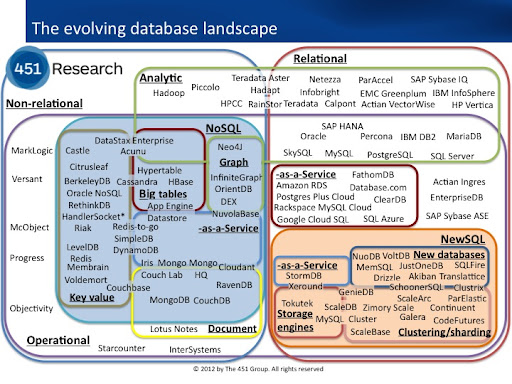
\includegraphics[width=.7\textwidth]{./imgs/dblandscape.jpg}
	\end{minipage}
	\caption{Схема современных категорий баз данных}
	\label{fig:dblandscape}
\end{figure}


Для хранения журналов чаще всего используются документо-ориентированные и колоночные базы данных,
поскольку они могут эффективно управлять гетерогенными и неструктурированными данными, характерными для журналов приложений.

Преимущества использования NoSQL баз данных для журнальных данных включают:

\begin{itemize}

	\item Гибкость схемы: Данные журналирования могут варьироваться по формату и структуре. NoSQL базы данных позволяют сохранять журналы без предварительного определения жесткой схемы.
	\item Масштабируемость: NoSQL базы данных хорошо масштабируются, позволяя обрабатывать большое количество операций записи, что часто требуется при журналировании.
	\item Оптимизация для чтения/записи: В зависимости от типа NoSQL базы данных можно оптимизировать операции записи (как в случае с колоночными и ключ-значение базами) или чтения (как в документо-ориентированных базах данных), что делает их высокопроизводительными для соответствующих типов нагрузок.
\end{itemize}

\subsection{Колоночные базы данных}

Концепция колоночных баз данных начала развиваться в 1970-х годах, но наибольшее распространение и развитие она получила в конце 1990-х – начале 2000-х годов благодаря росту объемов данных и потребности в их аналитике. Колоночное хранение данных было предложено как альтернатива традиционным реляционным базам данных с целью оптимизации скорости чтения данных и уменьшения затрат на хранение посредством компрессии.

Одной из первых систем, предложивших использование колоночного хранения данных, была Sybase IQ, которая была выведена на рынок в начале 1990-х годов.
Современные колоночные базы данных, такие как ClickHouse, Apache Cassandra, и Amazon Redshift, продолжают развивать идеи, заложенные их предшественниками, предлагая мощные возможности для управления и анализа больших данных с высокой скоростью и эффективностью. Область применения колоночных баз данных постоянно расширяется, охватывая такие задачи, как реальная обработка данных (real-time processing), интернет вещей (IoT), машинное обучение и многие другие.

Основная идея колоночных СУБД — это хранение данных не по строкам, как это делают традиционные СУБД, а по колонкам. Это означает, что с точки зрения SQL-клиента данные представлены как обычно в виде таблиц, но физически эти таблицы являются совокупностью колонок, каждая из которых по сути представляет собой таблицу из одного поля. При этом физически на диске значения одного поля хранятся последовательно друг за другом. Принцип хранения данных колоночными СУБД представлен на рисунке \ref{fig:columnarvsrelational}

\begin{figure}[H]
	\centering
	\begin{minipage}[t]{.9\textwidth}
		\centering
		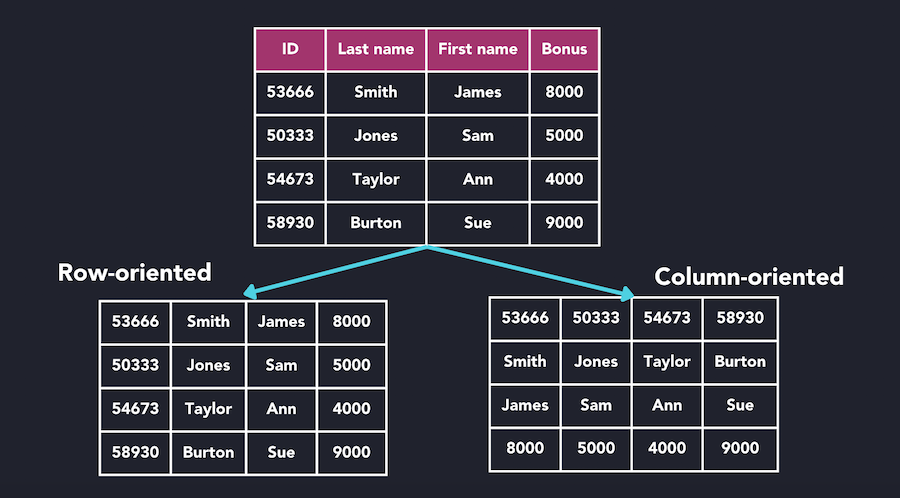
\includegraphics[width=.7\textwidth]{./imgs/columnar-database.png}
	\end{minipage}
	\caption{Различия реляционных и колоночных баз данных}
	\label{fig:columnarvsrelational}
\end{figure}


Организация хранения данных по столбцам дает следующие преимущества:

\begin{enumerate}
	\item Высокая степень сжатия данных. Хранение данных по столбцам позволяет применять более эффективные методы сжатия, так как каждый столбец содержит данные одного типа. Это уменьшает использование дискового пространства и улучшает производительность, так как читать и передавать данные становится быстрее. Одним из популярных алгоритмов является Run-Length Encoding (RLE): Если есть таблица со 100 млн записей, сделанных в течение одного года, то в колонке «Дата» на самом деле будет храниться не более 366 возможных значений, так как в году не более 366 дней (включая високосные года). Поэтому можно 100 млн отсортированных значений в этом поле заменить на 366 пар значений вида <дата, количество раз> и хранить их на диске в таком виде. При этом они будут занимать приблизительно в 100 тыс. раз меньше места, что также способствует повышению скорости выполнения запросов;
	\item Быстрая агрегация. Колоночные СУБД идеально подходят для выполнения агрегатных операций, таких как COUNT, SUM, AVG и т.д., поскольку эти операции могут выполняться непосредственно над данными внутри столбца без необходимости обращения к данным других столбцов;
	\item Улучшенный анализ больших данных. Благодаря высокому уровню сжатия и специализированной организации данных, колоночные СУБД особенно хороши для аналитики больших объемов данных;
	\item Легкость добавления новых столбцов. В колоночных базах данных добавление нового столбца обычно является более простой операцией и не влечет за собой дорогостоящих операций перестроения таблиц, в отличие от реляционных СУБД, где структура таблицы строгая и модификация схемы может быть более сложной.
\end{enumerate}


В настоящий момент существует множество СУБД, хранящих данные в колонках. Наиболее популярными являются:

\begin{enumerate}
	\item{Apache Cassandra. Была создана для инфраструктуры поиска Inbox. Apache Cassandra является проектом Apache Software Foundation. Преимущества:
	      \begin{itemize}
		      \item Высокая масштабируемость и надежность;
		      \item Децентрализованная архитектура, избегает "единой точки отказа";
		      \item Хорошо справляется с большими объемами данных.
	      \end{itemize}}
	\item{ClickHouse. Разработанная российской компанией Яндекс для аналитики веб-поиска, ClickHouse быстро набрала популярность благодаря своей отличной производительности и эффективности. Преимущества:
	      \begin{itemize}
		      \item Очень высокая скорость обработки запросов;
		      \item Эффективное сжатие данных;
		      \item Подходит для аналитики в реальном времени.
	      \end{itemize}}

	\item{Google Bigtable. Данная СУБД была разработана в качестве внутреннего инструмента в Google, Bigtable стала основой для таких продуктов, как поисковая система Google, Google Maps и Gmail. Преимущества:
	      \begin{itemize}
		      \item Высокая производительность и масштабируемость для обработки больших объемов данных;
		      \item Хорошо подходит для временных рядов, IoT и аналитических приложений;
		      \item Интеграция с сервисами Google Cloud.
	      \end{itemize}
	      }
	\item{Apache HBase. Разработана как часть проекта Hadoop для работы с большими наборами данных в распределенной вычислительной среде. Поддерживает весь стандарт Hadoop и его экосистему и предлагает возможности построения больших, масштабируемых и распределенных баз данных, способных обрабатывать миллиарды строк и миллионы столбцов. Преимущества:
	      \begin{itemize}
		      \item Интеграция с Hadoop экосистемой;
		      \item Поддержка хранения и обработки больших объемов данных;
		      \item Высокая производительность при случайном доступе к данным.
	      \end{itemize}
	      }


	\item{Vertica. Была разработана Майклом Стоунбрейкером и его командой, Vertica является коммерческой колоночной СУБД, которая была приобретена компанией HP в 2011 году. Она известна своей способностью обрабатывать данные в чрезвычайно больших объемах, своей производительностью, масштабируемостью и встроенными аналитическими функциями.}
\end{enumerate}


\subsection{База данных ClickHouse}

СУБД ClickHouse \cite{ClickDocs} изначально была разработана для поддержки Яндекс.Метрики
--- второй крупнейшей в мире платформы для веб-аналитики — и по-прежнему является её ключевым компонентом.
С более чем 13 триллионами записей в базе данных и более 20 миллиардами событий в сутки,
ClickHouse позволяет создавать на лету индивидуально настроенные отчёты напрямую из неагрегированных данных.

ClickHouse выделяется среди других колоночных баз данных благодаря своей высокой производительности
и скорости выполнения сложных аналитических запросов.
Он использует эффективные методы сжатия данных, такие как LZ4, Zstd и Brotli,
что уменьшает объем хранимых данных и ускоряет их обработку.
ClickHouse хорошо масштабируется горизонтально, позволяя добавлять
новые узлы в кластер для увеличения производительности.
Перечисленные преимущества говорят о том, что ClickHouse является
хорошим выбором для задачи хранения данных журналирования. Возможности быстрого поиска
и анализа данных позволяют эффективно обрабатывать миллиарды событий в день.
Проект с открытым исходным кодом обеспечивает активное развитие и поддержку
со стороны сообщества, благодаря чему появилость большое количество интеграция
с различными ЯП, инструментами визуализации и тд. Обзор инструментов представлен таблице \ref{table:clickhouse_tools}

\begin{table}[H]

	\caption{Инструменты для работы с ClickHouse}
	\centering
	\begin{tabularx}{\textwidth}{|l|l|X|}
		\hline
		\textbf{Категория}  & \textbf{Название} & \textbf{Описание}                                                                         \\ \hline
		Языковой клиент     & Go                & Нативный интерфейс GO для подключения к ClickHouse                                        \\ \hline
		Языковой клиент     & Java              & Java-клиент для ClickHouse                                                                \\ \hline
		Языковой клиент     & Python            & Набор пакетов Python для подключения к ClickHouse                                         \\ \hline
		Ввод данных         & Amazon S3         & Извлечение, загрузка и преобразование данных из S3-бакетов                                \\ \hline
		Ввод данных         & Redpanda          & Платформа потоковых данных для вставки данных в режиме реального времени                  \\ \hline
		Ввод данных         & dbt               & Пакет dbt для преобразования данных в ClickHouse                                          \\ \hline
		Ввод данных         & Apache Airflow    & Платформа управления рабочими процессами с открытым исходным кодом                        \\ \hline
		Визуализация данных & Superset          & Инструмент визуализации данных, идеально подходящий для создания панелей потоковых данных \\ \hline
		Визуализация данных & Grafana           & Инструмент пользовательского интерфейса с открытым исходным кодом для визуализации данных \\ \hline
		Визуализация данных & Explo             & Инструмент визуализации данных для аналитики в реальном времени                           \\ \hline
		SQL-клиент          & ClickHouse Client & Нативный консольный клиент для ClickHouse                                                 \\ \hline
		SQL-клиент          & DataGrip          & IDE для работы с базами данных со специализированной поддержкой ClickHouse                \\ \hline
		SQL-клиент          & JupySQL           & Нативный SQL-клиент для Jupyter Notebooks                                                 \\ \hline
	\end{tabularx}
	\label{table:clickhouse_tools}
\end{table}

На рисунке \ref{fig:clickbench} представлены результаты сравнения производительности ClickHouse и других популярных БД \cite{ClickBench}.


\begin{figure}[H]
	\centering
	\begin{minipage}[t]{.9\textwidth}
		\centering
		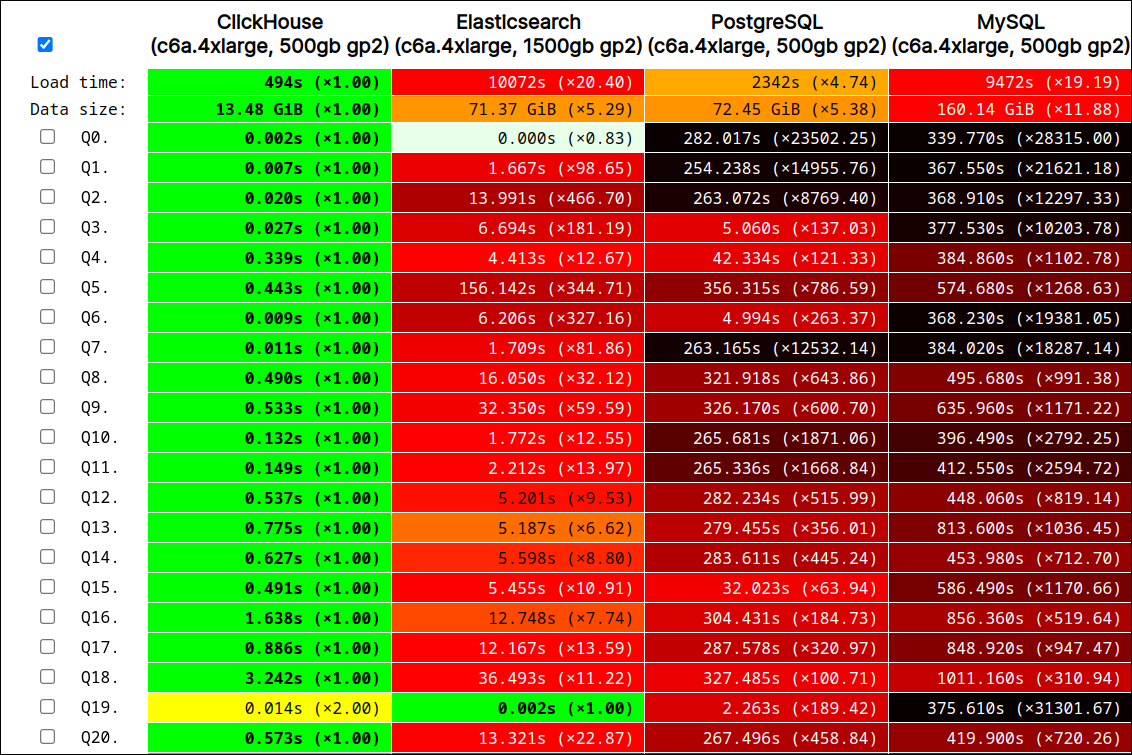
\includegraphics[width=.7\textwidth]{./imgs/clickbench.png}
	\end{minipage}
	\caption{Сравнение производительности ClickHouse c другими СУБД}
	\label{fig:clickbench}
\end{figure}

Производительность измерялась на запросах, использующих агрегирующие функции, такие как: COUNT, SUM, AVG и тд. Как видно из результатов, ClickHouse
выигрывает по скорости популярные реляционные базы данных. В тесте 19 видно, что ClickHouse уступает Elasticsearch. Данный результат ожидаем,
так как в этом тесте используется запрос представленный на листинге \ref{lst:elasticwin_query}.

\begin{listing}[H]
	\caption{Запрос для тестирования производительности ClickHouse}
	\label{lst:elasticwin_query}
	\inputminted[style=bw, frame=single,fontsize = \footnotesize, linenos=false, xleftmargin = 1.5em]{SQL}{./listings/elastic_win.sql}
\end{listing}

В данном запросе используется условие выбора по точному совпадению. В этом случае выигрывает Elasticsearch,
т.к. по-умолчанию в этой СУБД строится поисковый индекс.

Таким образом, ClickHouse является обоснованным выбором для
организации хранения данных журналов приложений.
Данная система позволит не только эффективно хранить лог-сообщения, но и быстро строить по ним
аналитику.


\section{Разработка приложения}

Для разработки приложения необходимо продумать схему доставки данных от приложений
до хранилища. Получившееся приложение должно обечивать надежность
для доставляемых данных, а также возможность горизонтального масшатабирования.


\subsection{Архитектура приложения}

Ключевым моментом архитектры данного приложения
является использование брокера сообщений. Такое решение
позволяет обеспечить отказоустойсивость и надежность.
При нарушении работы приложения, данные от клиентов будут сохранены в брокере,
кроме того, некоторые брокеры сохраняют сообщеня даже после их прочтения,
примером является Apache Kafka. Использование брокера
сообщений позволяет также горизонтально масштабировать
разрабатываемое приложение, добавляя его копии в качестве
слушаталей к активным очередям сообщений. Кроме того,
такое решение позволит интегрироваться с существующими
агентами сбора данных приложений, например  Fluentd, Fluent-bit.
Эти агенты поддерживают отправку данных в различные источники, в том
числе очереди сообщений. Схема работы агента Fluent-bit представлена на
рисунке \ref{fig:fluentbitscheme}

\begin{figure}[H]
	\centering
	\begin{minipage}[t]{.9\textwidth}
		\centering
		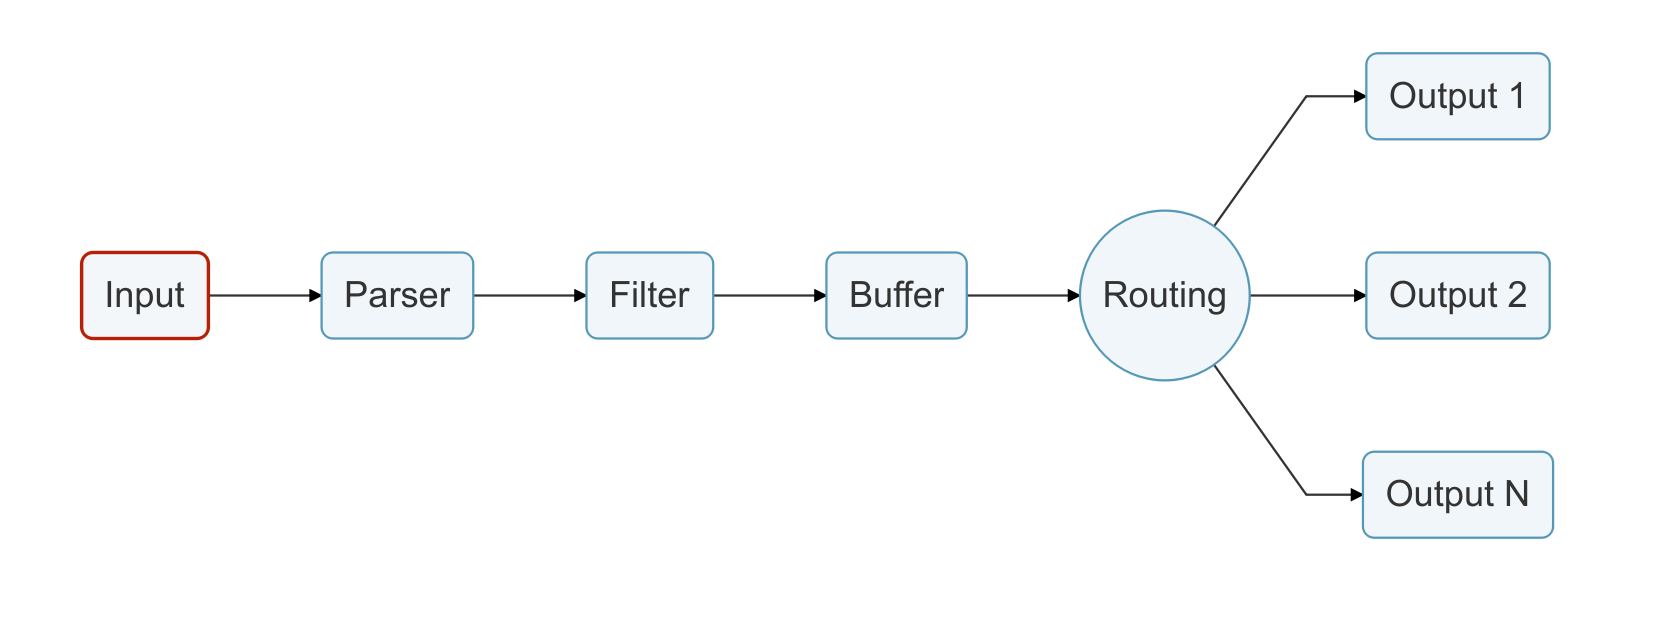
\includegraphics[width=.7\textwidth]{./imgs/fluentbit.png}
	\end{minipage}
	\caption{Схема работы агента Fluent-Bit}
	\label{fig:fluentbitscheme}
\end{figure}

Описание схемы работы Fluent-bit

\begin{enumerate}
	\item Получение входных данных. Fluent-Bit начинает свою работу с чтения данных из различных источников. Это могут быть:
	      \begin{itemize}
		      \item Лог-файлы на файловой системе;
		      \item Стандартные потоки вывода (stdout) приложений;
		      \item Сетевые порты для приема данных по протоколам TCP или UDP;
		      \item Другие источники, такие как systemd журналы, Windows Event Log и т.д.
	      \end{itemize}

	\item Обработка и фильтрация. Полученные данные проходят через этап обработки и фильтрации. Fluent-Bit поддерживает различные фильтры, которые позволяют обрабатывать и структурировать данные перед их отправкой. Например:
	      \begin{itemize}
		      \item Разделение сообщений: разбиение входящих данных на отдельные сообщения;
		      \item Разбор формата: извлечение полей из структурированных лог-сообщений (например, JSON или CSV);
		      \item Преобразование данных: изменение или расширение данных;
		      \item Отбрасывание данных: исключение определенных сообщений на основе заданных условий.
	      \end{itemize}

	\item Буферизация. Fluent-Bit поддерживает механизмы буферизации данных, которые обеспечивают надежную доставку данных в случае временных сбоев или недоступности целевого хранилища данных (например, сервера логов или метрик). Буферизация позволяет временно сохранять данные и повторно пытаться отправить их позже.

	\item Отправка данных.
	      После обработки и, возможно, буферизации данных, Fluent-Bit отправляет их в целевое хранилище или аналитическую систему.

\end{enumerate}



Итоговая архитектура приложения изображена на рисуке \ref{fig:appscheme}.

\begin{figure}[H]
	\centering
	\begin{minipage}[t]{.9\textwidth}
		\centering
		
\includegraphics[width=.7\textwidth]{./imgs/appscheme.png}
	\end{minipage}
	\caption{Схема работы приложения}
	\label{fig:appscheme}
\end{figure}


Между брокером и базой данных есть промежуточный элемент. Это приложение,
которые необходимо разработать. Этот слой позволяет
внедрить дополнительный функционал, например:

\begin{itemize}
	\item Проверка лог-сообщений на критические данные и их маскирование;
	\item Обогащение данными из других источников;
	\item
	\item
\end{itemize}

Одной из важных особенностей данного слоя является организация
множественной вставки. Т.е. необходимо накапливать
какое-то количество сообщений перед вставкой.
Иначе использование ClickHouse будет неоправданнным, т.к.
наиболее производительными являются запросы на множественную
вставку. В документации ClickHouse \cite{ClickDocs} указано, что данные
рекомендуется вставлять пачками не менее 1000 строк
или не более одного запроса в секунду.

\subsection{Выбор инструментов разработки}

Для разработки приложбыл выбран язык Golang \cite{Golang} из-за следующих его преимуществ:

\begin{itemize}
	\item Высокая производительность. Golang компилируется в машинный код, что обеспечивает высокую производительность;
	\item Go имеет встроенную поддержку многопоточности через горутины, которые являются легковесными потоками. Это позволяет легко обрабатывать множество параллельных задач, таких как чтение сообщений из очереди и запись их в базу данных, без значительных затрат на управление потоками;
	\item Go предоставляет богатую стандартную библиотеку, включающую поддержку сетевых операций, работы с файлами и взаимодействия с различными базами данных;
	\item Существует нативный клиент для Go, который обеспечивает эффективное и удобное взаимодействие с ClickHouse. Это позволяет быстро и надежно записывать лог-сообщения в базу данных, используя преимущества производительности ClickHouse;
	\item Go хорошо подходит для работы с различными системами очередей, такими как Apache Kafka или RabbitMQ, благодаря своей многопоточности и производительности. Это позволяет эффективно обрабатывать входящие сообщения и записывать их в ClickHouse без значительных задержек.
\end{itemize}

В качестве очереди сообщение будет использована Apache Kafka. Kafka сохраняет
все сообщения в распределенном журнале,
который можно настроить для долговременного хранения данных. Это позволяет обеспечить
дополнительную надежность при обработке данных. Также Kafka поддерживает репликацию данных на несколько брокеров,
что обеспечивает высокую доступность и устойчивость к сбоям.
Если один брокер выходит из строя, другой брокер с репликой данных может взять на себя его роль,
обеспечивая непрерывность работы системы.

Для взаимодействия с кластером Apache Kafka небходимо выбрать драйвер языка Golang.
Самыми популярными являются:

\begin{itemize}
	\item Sarama;
	\item Confluent Kafka Golang Client;
	\item Kafka-go;
	\item Franz-go.
\end{itemize}


В проекте будет использоваться Sarama. Так как
это нативная библиотека, которая имеет хорошую
документацию и активное сообщество.


\section{Реализация приложения}

Для реализации приложения
необходимо настроить
кластера для Apache Kafka
и ClickHouse, а также
реализовать приложение-посредник
для доставки сообщений из очереди
сообщений в постоянное хранилище


Для простоты разработки все части
реализумого приложения будут разворачиваться
в Docker \cite{DockerDocs} контейнерах. Для организации
взаимодействия между контейнерами будет
использоваться Docker Compose \cite{DockerComposeDocs}.

\subsection{Настройка Apache Kafka}

Первоночально, необходимо выбрать образ с Apache Kafka.
Самым популярным является bitnami/kafka. На данный
момент насчитывается более ста миллионов скачиваний данного образа
с hub.docker.com. Кроме того, для удобного
управления кластером, можно воспользоваться
приложением, предоставляющим веб-интерфейс для
Apache Kafka. В нем можно отслеживать информацию об существующих очередях
Управлять топиками и сообщениями. Пример интерфейса приведен на рисунке \ref{fig:kafkaui}.

\begin{figure}[H]
	\centering
	\begin{minipage}[t]{.9\textwidth}
		\centering
		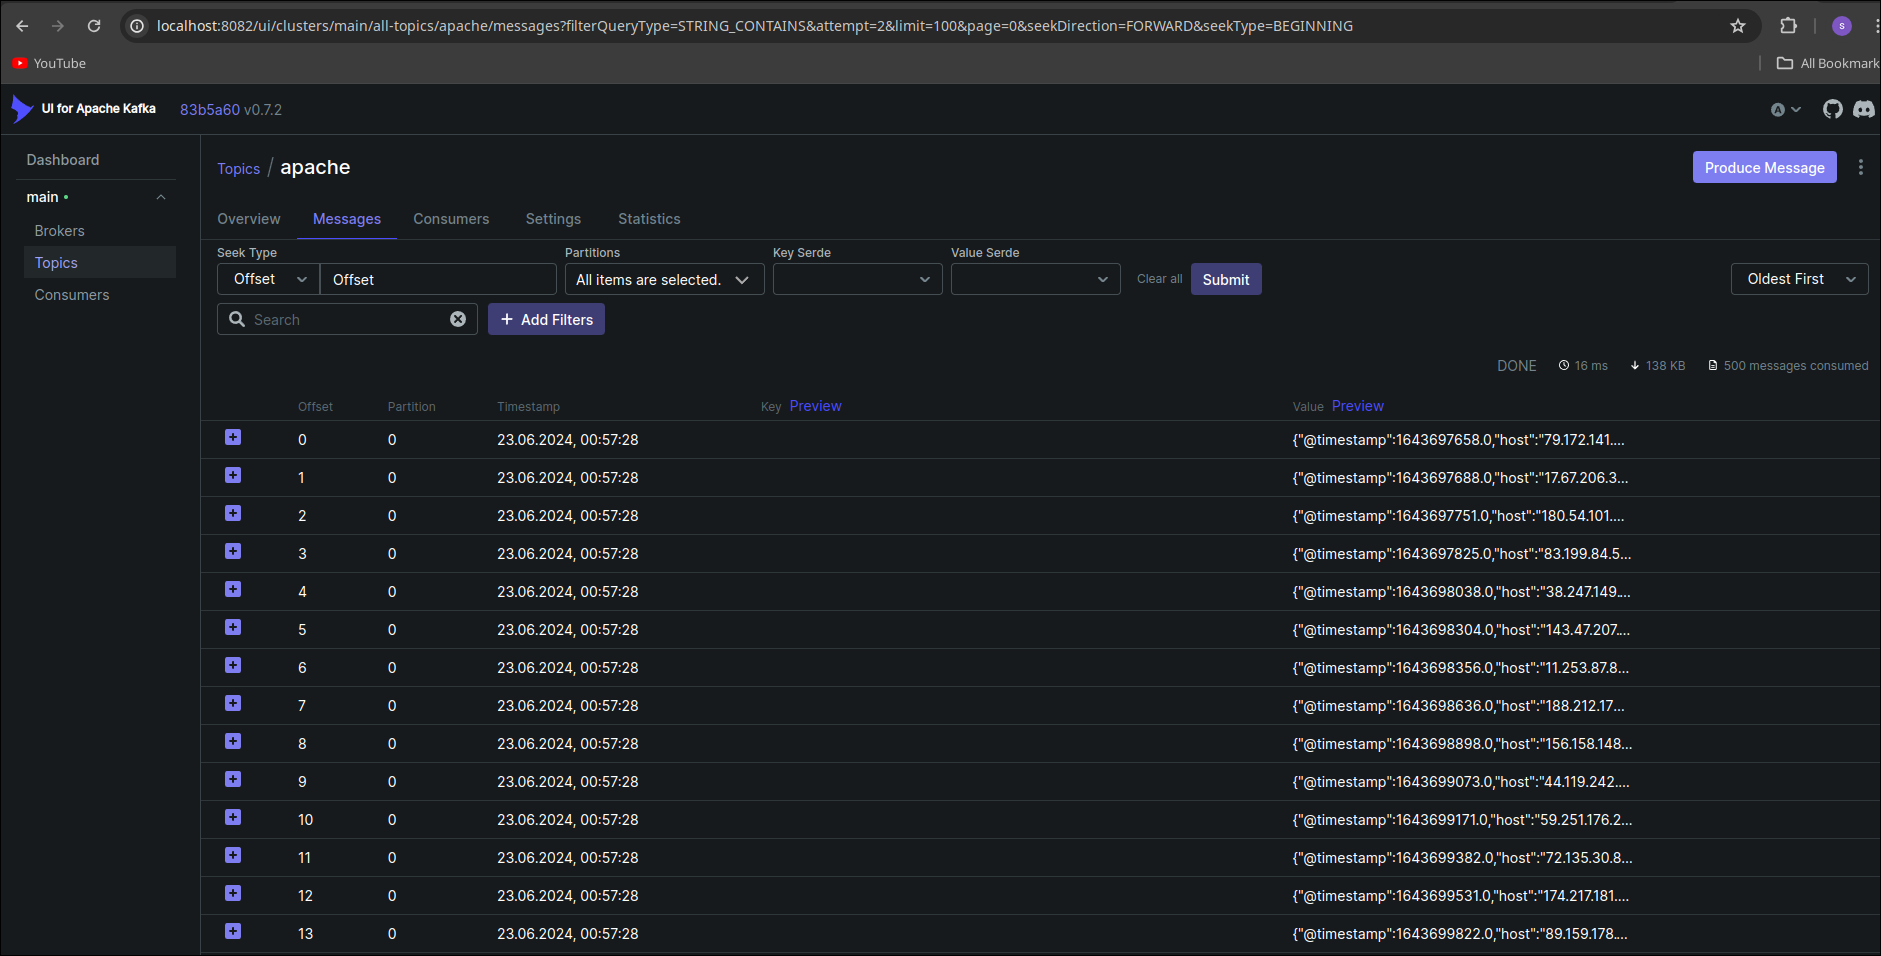
\includegraphics[width=.7\textwidth]{./imgs/kafkaui.png}
	\end{minipage}
	\caption{Схема современных категорий баз данных}
	\label{fig:kafkaui}
\end{figure}

За веб-интерфейс будет отвечать образ provectuslabs/kafka-ui.
После подключения кластера в веб-интерфейсе, появится возможность
в реальном времени отслеживать поток сообщений в очереди,
состояния получателей, а также отсылать тестовые сообщения.

Конфигурация Apache Kafka представлена на листинге \ref{lst:dockerkafka}

\begin{listing}[H]
	\caption{Описание сервиса Apache Kafka в Docker Compose}
	\label{lst:dockerkafka}
	\inputminted[style=bw, frame=single,fontsize = \footnotesize, linenos=false, xleftmargin = 1.5em]{yaml}{./listings/kafka.yml}
\end{listing}


\subsection{Настройка Clickhouse}

В качестве образа для ClickHouse используется образ от той же организации bitnami.
ClickHouse имеет несколько интерфейсов взаимодействия:
\begin{enumerate}
	\item Нативный протокол. Расположен на порте 9000. Используется приложениями и процессами ClickHouse, такими как clickhouse-server, clickhouse-client и встроенными инструментами ClickHouse. Также зайдействован для межсерверного взаимодействия при распределенных запросах.
	      Используется драйвером Golang для взаимодействия с СУБД;
	\item HTTP интерфейс. Расположен на порте 8123. Необходим для взаимодествия посредстом IDE. Например,
	      IDE DataGrip взаимодействует с ClickHouse посредство HTTP интерфейса.
\end{enumerate}

Конфигурация ClickHouse представлена на листинге \ref{lst:dockerclick}

\begin{listing}[H]
	\caption{Описание сервиса ClickHouse в Docker Compose}
	\label{lst:dockerclick}
	\inputminted[style=bw, frame=single,fontsize = \footnotesize, linenos=false, xleftmargin = 1.5em]{yaml}{./listings/clickhouse.yml}
\end{listing}

\subsection{Реализация приложения-посредника}

Для того чтобы задавать отслеживаемые очереди необходимо
разработать какой-либо интерфейс, например, REST, gRPC, JSON-RPC и тд.
Данный интерфейс должен предоставлять возможности добавления нового
источника данных. В качестве интерфейса взаимодействия
с приложением был выбран REST. Для реализации REST API использован
веб-фреймворк gin-gonic \cite{GinGonic}. На основе фреймворка
было спроектирована API в формате Swagger, которое представлено на
рисунке \ref{fig:api}

\begin{figure}[H]
	\centering
	\begin{minipage}[t]{.9\textwidth}
		\centering
		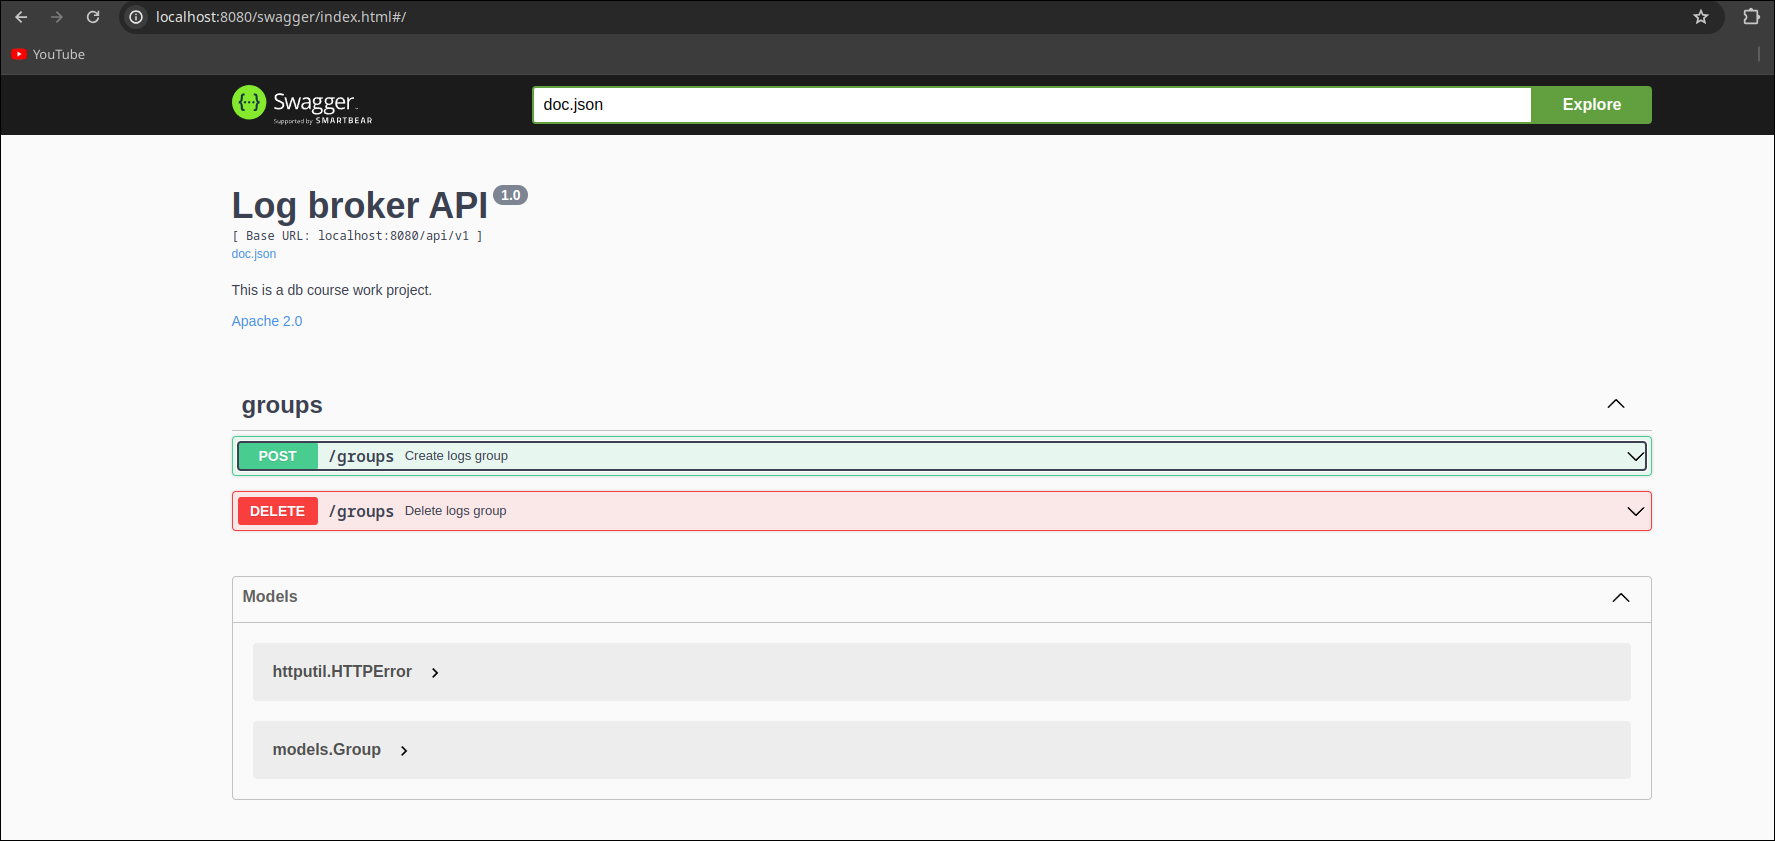
\includegraphics[width=.7\textwidth]{./imgs/swagger.png}
	\end{minipage}
	\caption{API приложения в формате Swagger}
	\label{fig:api}
\end{figure}

Данное API позволяет динамически менять отлеживаемые
очереди без необходимости перезапуска
приложения.

На листинге \ref{lst:groupadd} представлен пример запроса с помощью приложения httpie.

\begin{listing}[H]
	\caption{Добавление нового отслеживаемого источника}
	\label{lst:groupadd}
	\inputminted[style=bw, frame=single,fontsize = \footnotesize, linenos=false, xleftmargin = 1.5em]{shell}{./listings/group.sh}
\end{listing}

После отправки POST запроса по пути api/v1/group приложение начнет
отслеживать очередь с указанным в запросе названием. На рисунке \ref{fig:groupadding}
показан журнал приложения, на котором видно, что в после получнея POST запрос
был добавлен новый источник для отслеживания, а именно очередь под названием
apache.

\begin{figure}[H]
	\centering
	\begin{minipage}[t]{.9\textwidth}
		\centering
		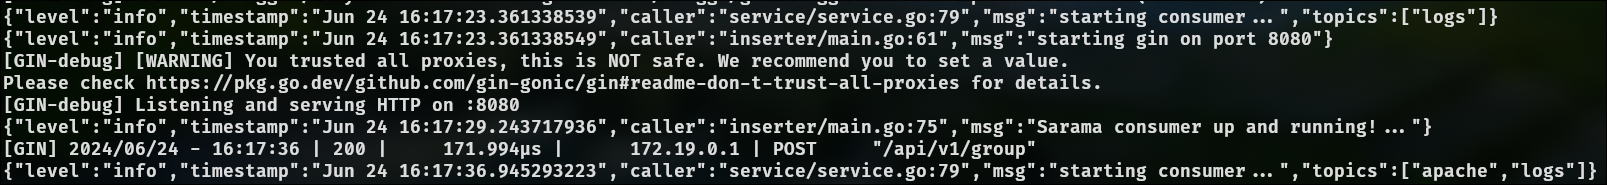
\includegraphics[width=.7\textwidth]{./imgs/addedgroup.png}
	\end{minipage}
	\caption{Результат добавления нового источника данных}
	\label{fig:groupadding}
\end{figure}


API и слушатель очереди работают в разных потоках. Для общения между потоками
используется объект типа context.Context. Благодря ему можно отправить сообщение
другому потоку. Воторой поток в свою очередь
обработает полученный сигнал. Если полученный сигнал
содержит ошибку, значит необходимо завершить работу всего приложения, иначе
данный сигнал свидетельствует об изменении конфигурации приложение, например, об
добавлении новой очереди для прослушивания. Логика с отправкой сигнала потоку
со слушателем очередей расположена в листинге \ref{lst:ctxclosing}.

\begin{listing}[H]
	\caption{Добавление нового источника данных}
	\label{lst:ctxclosing}
	\inputminted[style=bw, frame=single,fontsize = \footnotesize, linenos=false, xleftmargin = 1.5em]{shell}{./listings/contextclose.go}
\end{listing}

Перед тем, как подать сигнал происходит обновление множества
прослушиваемых очередей.

На листинге \ref{lst:consumerctx} код запуска слушателя очередей.
Данный слушатель запускается синхронно, т.е. код блокируется в 
вызове функции s.client.Consume. После выхода 
из функции происходит обработка причины выхода. Если 
не произшло ошибок, то данная функция вызовется снова, иначе
в журнал будет записано сообшение об ошибке и приложение завершит работу.

\begin{listing}[H]
	\caption{Запуск слушателя очередей}
	\label{lst:consumerctx}
	\inputminted[style=bw, frame=single,fontsize = \footnotesize, linenos=false, xleftmargin = 1.5em]{shell}{./listings/consumerctx.go}
\end{listing}

На листинге \ref{lst:dockerinserter} содержится описание приложения-посредника.

\begin{listing}[H]
	\caption{Описание сервиса посредника в Docker Compose}
	\label{lst:dockerinserter}
	\inputminted[style=bw, frame=single,fontsize = \footnotesize, linenos=false, xleftmargin = 1.5em]{yaml}{./listings/inserter.yml}
\end{listing}

Реализация взаимодействия с ClickHouse представлена на листинге 
Каждому источнику данных соответствует таблица с двумя полями:

\begin{itemize}
  \item Поле timestamp типа DateTime64. Время вставки сообщения в таблицу;
  \item Поле payload типа JSON. Данное поле и хранит все содержимое сообщения в формате JSON.
\end{itemize}

Долгое время, в ClickHouse тип JSON был синонимом строкового типа. Т.е. использование этого типа 
не давало никакого преимущества, а для работы с такими полями использовались специальные функции, которые 
позволяли извлекать значения определенных полей.
Начиная с версии 22.3 тип JSON был обновлен, и перестал быть просто синонимом строкового типа.

Схема обработки представлена на рисунке \ref{fig:jsonprocessing}. 

\begin{figure}[H]
	\centering
	\begin{minipage}[t]{.9\textwidth}
		\centering
		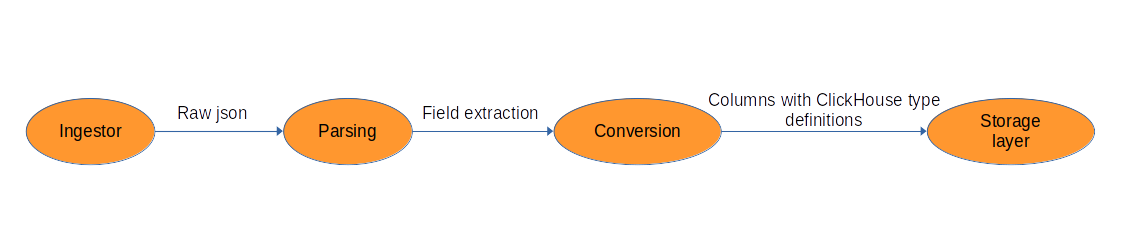
\includegraphics[width=.7\textwidth]{./imgs/ingestion_process_crop.png}
	\end{minipage}
	\caption{Обработка значения типа JSON в ClickHouse версии 22.3}
	\label{fig:jsonprocessing}
\end{figure}

Начиная с версии 22.3 все значения типа JSON проходят
этап извлечения значений и присвоения определенных типов,
после чего для каждого поля создается отдельный столбец.

Рассмотрим данный механизм на примере. Создание таблицы подобной 
схемы представлено на листинге \ref{lst:jsontable}. 


\begin{listing}[H]
	\caption{Создание таблицы с полем типа JSON}
	\label{lst:jsontable}
	\inputminted[style=bw, frame=single,fontsize = \footnotesize, linenos=false, xleftmargin = 1.5em]{sql}{./listings/jsontable.sql}
\end{listing}

Функционал хранения данных в JSON является экспериментальным, поэтому
необходимо установить переменную allow\_experimental\_object\_type в единицу.
На листинге \ref{lst:insertjson} представлен запрос
на вставку строки в JSON формате

\begin{listing}[H]
	\caption{Вставка JSON строки}
	\label{lst:insertjson}
	\inputminted[style=bw, frame=single,fontsize = \footnotesize, linenos=false, xleftmargin = 1.5em]{sql}{./listings/inserjson.sql}
\end{listing}

Теперь, небходимо выполнить запрос DESCRIBE, который
покажет, в каком формате хранится значение. Результат
данного запроса представлен на рисунке \ref{fig:descres}. 

\begin{figure}[H]
	\centering
	\begin{minipage}[t]{.7\textwidth}
		\centering
		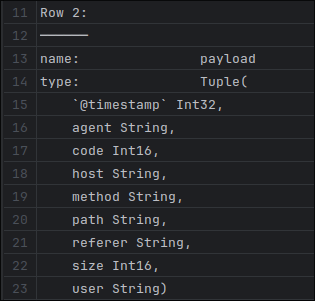
\includegraphics[width=.6\textwidth]{./imgs/descres1.png}
	\end{minipage}
	\caption{Обработка значения типа JSON в ClickHouse версии 22.3}
	\label{fig:descres}
\end{figure}

Как видно из рисунка, поле payload является не строкой,
а кортежем различных значений, как числовых так и строковых.

\section{Тестирование приложения}

\renewcommand\refname{СПИСОК ИСПОЛЬЗОВАННЫХ ИСТОЧНИКОВ}
% Список литературы
\clearpage
%\bibliographystyle{ugost2008s}  %utf8gost71u.bst} %utf8gost705u} %gost2008s}
{\catcode`"\active\def"{\relax}
\addcontentsline{toc}{section}{\protect\numberline{}\refname}%
%\bibliography{biblio} %здесь ничего не меняем, кроме, возможно, имени bib-файла
\printbibliography
}
\newpage
\settocdepth{section}
\anonsection{ПРИЛОЖЕНИЕ А}
\vspace{-30pt}


\end{document}
